%----------------------------------------------------------------------------
\chapter{Verifikáció}
\label{sec:verifikacio}

%----------------------------------------------------------------------------
\section{A {\thetaSc} tesztelése}
%----------------------------------------------------------------------------
Az egyes elemeknek egyenlőre nem készültek Unit tesztjeik.

A szerializációt több különböző állapotgépre is lefuttattam, kipróbálva minden elemet. Erre egy példa van a \hyperref[fig:serializeexample]{3.4} és a \hyperref[fig:serializeresult]{3.5-ös} ábrán.
Erre egy teszt osztály a \verb+ParserTest+, ami beolvas egy sorosított állapotgépet, majd kiírja a standard output-ra


%----------------------------------------------------------------------------
\section{A transzformáció tesztelése}
%----------------------------------------------------------------------------
Több állapotgépet is létrehoztam Yakindu-ban, ezeket a Gamma Framework segítségével {\gammaSc}pé alakítottam. Ezekkel az állapotgép modellekkel futtattam a \verb+ConverterTest+ tesztet, ami {\thetaSc}pé transzformálja a kapott Gamma modellt. A \hyperref[fig:serializeexample]{3.4-es ábrán} látható állapotgép is így lett {\thetaSc}pé konvertálva és utána sorosítva.


%----------------------------------------------------------------------------
\section{Az állapotgép konfiguráció tesztelése}
%----------------------------------------------------------------------------
A \verb+StateConfigurationTester+ osztállyal teszteltem az állapotgép konfigurációt. A \hyperref[fig:configexample]{7.1-es ábrán} átható az állapotgép, amin futtattam a tesztet. A következő tranzíciókat tüzeljük el: 
\begin{enumerate}
	\item StateA --> Ortogonal
	\item B --> E
	\item G --> H
	\item Ortogonal --> StateA
	\item StateA --> Ortogonal
\end{enumerate}

Ezek után a következő állapotoknak kell aktívnak lennie:
\begin{itemize}
	\item CompositeA,
	\item CompositeB,
	\item G mert a history megjegyezte, hogy kilépéskor CompositeA volt aktív, viszont az azon belüli állapotot már nem jegyezte meg tehát hiába volt H aktív, most már újra G-az,
	\item E, mert a deep history azt is megjegyezte, hogy CompositeB-n belül mi volt az aktív állapot
	\item Ortogonal
\end{itemize}

A teszt sikeresen lefutott.

\begin{figure}[!ht]
	\centering
	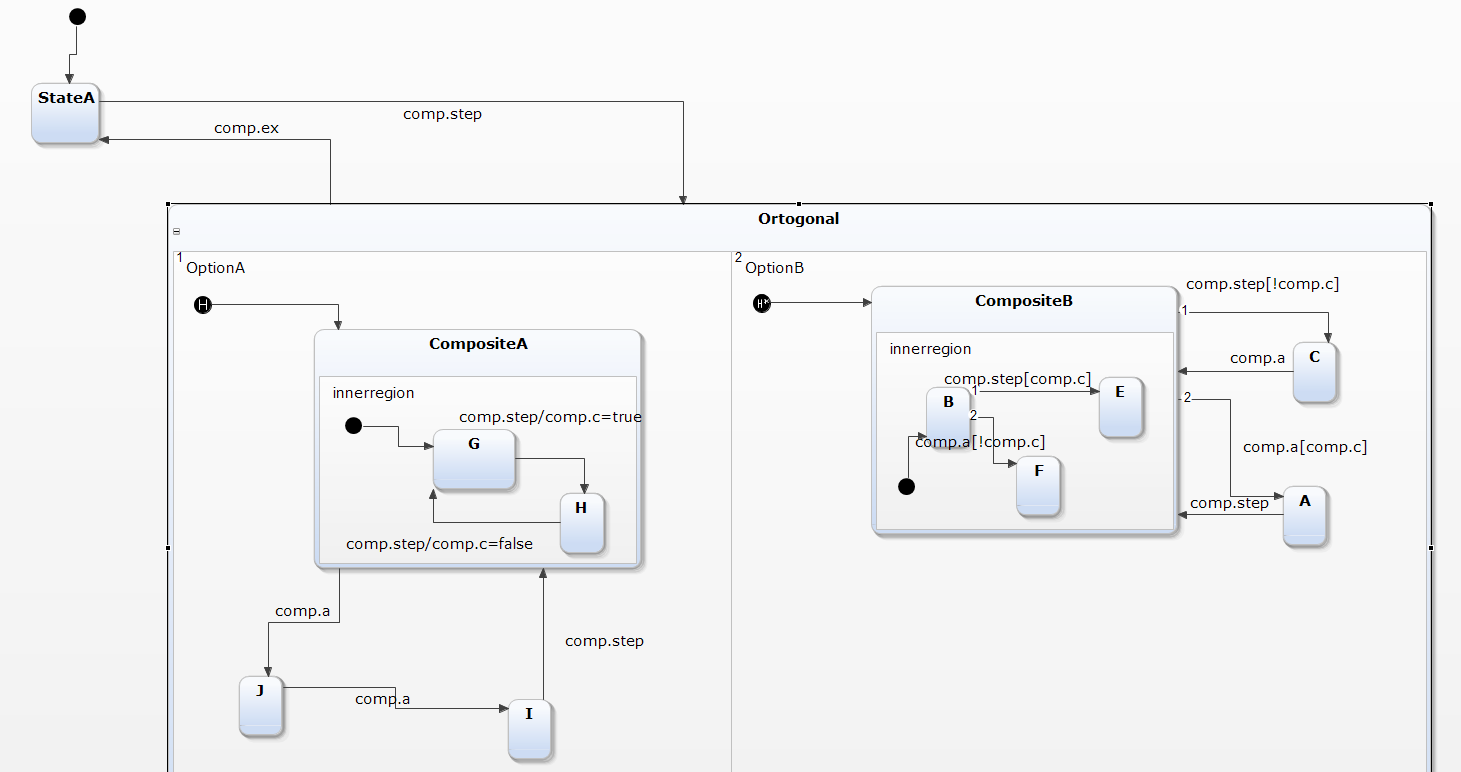
\includegraphics[width=150mm, keepaspectratio]{figures/komplex.png}
	\caption{Az állapotgép, amin a konfigurációs tesztet végeztem}
	\label{fig:configexample}
\end{figure}

%----------------------------------------------------------------------------
\section{A BMC tesztelése}
%----------------------------------------------------------------------------
A \verb+BoundedCheckerTest+ osztállyal lehet beolvasott {\thetaSc}eken tesztelni. Például a \hyperref[fig:serializeexample]{3.4-es állapotgépen} keresve az F hiba állapotot. A \hyperref[fig:bmcresult]{következő eredményt kapjuk:} 

\begin{figure}[!ht]
	\centering
	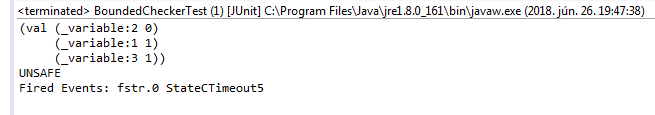
\includegraphics[width=150mm, keepaspectratio]{figures/bmcresult.png}
	\caption{A BoundedCheckerTest futási eredménye}
	\label{fig:bmcresult}
\end{figure}

Itt láthatjuk, hogy a solver által vissza adott példában három különböző változó szerepel, pedig csak egy változó van az állapotgépben. A másik kettő az új értékadás után jött létre. Az \verb+UNSAFE+ azt jelenti, az F állapot elérhető. Utána felsorolásként ott vannak azok az események, amik kiváltják a szükséges tranzíciókat. Viszont az időzítési feltételeket egyenlőre nem vizsgáljuk, ez a jövőbeni tervek közé tartozik.

